% !TEX encoding = UTF-8 Unicode

%%%%%%%%%%%%%%%%%%%%%%%%%%%%%%%%%%%%%%%%%%%%%%%%%%%%%%%%%%%%%%%%%%%%%%%%%%%%%%%%
% 																			   %
% Git Branch: master														   %
% 																			   %
%%%%%%%%%%%%%%%%%%%%%%%%%%%%%%%%%%%%%%%%%%%%%%%%%%%%%%%%%%%%%%%%%%%%%%%%%%%%%%%%

\pdfoutput=1 % to upload to arXiv with the hyperref package

\documentclass[10pt,twocolumn,twoside]{IEEEtran}

% Some very useful LaTeX packages include:
% (uncomment the ones you want to load)


% *** MISC UTILITY PACKAGES ***
%
%\usepackage{ifpdf}
% Heiko Oberdiek's ifpdf.sty is very useful if you need conditional
% compilation based on whether the output is pdf or dvi.
% usage:
% \ifpdf
%   % pdf code
% \else
%   % dvi code
% \fi
% The latest version of ifpdf.sty can be obtained from:
% http://www.ctan.org/pkg/ifpdf
% Also, note that IEEEtran.cls V1.7 and later provides a builtin
% \ifCLASSINFOpdf conditional that works the same way.
% When switching from latex to pdflatex and vice-versa, the compiler may
% have to be run twice to clear warning/error messages.

% Defines a paragraph counter ----------------------------------------------

\usepackage{chngcntr} % To reset counter at each section


% Paragraph counter 
\newcounter{para}
\newcommand\mypara{\par \thesection.\refstepcounter{para}\thepara.\space}

\counterwithin*{para}{section} % Resets counter at each section

% *** FONT AND LANGUAGE PACKAGES ***

\usepackage[utf8]{inputenc}
\usepackage[english]{babel}
\usepackage{mathrsfs} 

\usepackage{enumerate}

% *** CITATION PACKAGES ***
%
%\usepackage{cite}
% cite.sty was written by Donald Arseneau
% V1.6 and later of IEEEtran pre-defines the format of the cite.sty package
% \cite{} output to follow that of the IEEE. Loading the cite package will
% result in citation numbers being automatically sorted and properly
% "compressed/ranged". e.g., [1], [9], [2], [7], [5], [6] without using
% cite.sty will become [1], [2], [5]--[7], [9] using cite.sty. cite.sty's
% \cite will automatically add leading space, if needed. Use cite.sty's
% noadjust option (cite.sty V3.8 and later) if you want to turn this off
% such as if a citation ever needs to be enclosed in parenthesis.
% cite.sty is already installed on most LaTeX systems. Be sure and use
% version 5.0 (2009-03-20) and later if using hyperref.sty.
% The latest version can be obtained at:
% http://www.ctan.org/pkg/cite
% The documentation is contained in the cite.sty file itself.

%\usepackage[natbib=true,backend=biber,style=ieee,
%firstinits=true,doi=false,eprint=false,isbn=false,url=false,texencoding=utf8,bibencoding=utf8]{biblatex}
%\addbibresource[location=remote]{https://www.dropbox.com/s/r00o9lw76cksxvj/Library.bib?dl=1} 
%\AtBeginBibliography{\small}

% !!!! IF FILE NOT FOUND DOWNLOAD IT FROM
%https://www.dropbox.com/s/r00o9lw76cksxvj/Library.bib?dl=1




% *** GRAPHICS RELATED PACKAGES ***
%
\ifCLASSINFOpdf
  \usepackage{xcolor}
  \usepackage[pdftex]{graphicx}
  % declare the path(s) where your graphic files are
  \graphicspath{{./imgs/}}
  % and their extensions so you won't have to specify these with
  % every instance of \includegraphics
  \DeclareGraphicsExtensions{.pdf,.jpeg,.png}
  
 
  
  \usepackage{epstopdf} % Must be loaded right after graphicx
\else
  % or other class option (dvipsone, dvipdf, if not using dvips). graphicx
  % will default to the driver specified in the system graphics.cfg if no
  % driver is specified.
  % \usepackage[dvips]{graphicx}
  % declare the path(s) where your graphic files are
  % \graphicspath{{../eps/}}
  % and their extensions so you won't have to specify these with
  % every instance of \includegraphics
  % \DeclareGraphicsExtensions{.eps}
\fi
% graphicx was written by David Carlisle and Sebastian Rahtz. It is
% required if you want graphics, photos, etc. graphicx.sty is already
% installed on most LaTeX systems. The latest version and documentation
% can be obtained at: 
% http://www.ctan.org/pkg/graphicx
% Another good source of documentation is "Using Imported Graphics in
% LaTeX2e" by Keith Reckdahl which can be found at:
% http://www.ctan.org/pkg/epslatex
%
% latex, and pdflatex in dvi mode, support graphics in encapsulated
% postscript (.eps) format. pdflatex in pdf mode supports graphics
% in .pdf, .jpeg, .png and .mps (metapost) formats. Users should ensure
% that all non-photo figures use a vector format (.eps, .pdf, .mps) and
% not a bitmapped formats (.jpeg, .png). The IEEE frowns on bitmapped formats
% which can result in "jaggedy"/blurry rendering of lines and letters as
% well as large increases in file sizes.
%
% You can find documentation about the pdfTeX application at:
% http://www.tug.org/applications/pdftex


% *** CROSS-REF PACKAGES ***

\usepackage[hyperindex,breaklinks]{hyperref}% backref linktocpage pagebackref
%
\hypersetup{
% Uncomment the line below to remove all links (to references, figures, tables, etc)
%draft, 
colorlinks=true, linktocpage=true, pdfstartpage=1, pdfstartview=FitV,
% Uncomment the line below if you want to have black links (e.g. for printing black and white)
%colorlinks=false, linktocpage=false, pdfborder={0 0 0}, pdfstartpage=3, pdfstartview=FitV, 
breaklinks=true, pdfpagemode=UseNone, pageanchor=true, pdfpagemode=UseOutlines,
plainpages=false, bookmarksnumbered, bookmarksopen=true, bookmarksopenlevel=1,
hypertexnames=true, pdfhighlight=/O, urlcolor=red!50!black, linkcolor=green!50!black, citecolor=green!50!black,
%
% PDF file meta-information
%
pdftitle={},
pdfauthor={},
pdfsubject={},
pdfkeywords={},
pdfcreator={},
pdfproducer={LaTeX}
}



% *** MATH PACKAGES ***
%
\usepackage{amsmath, amsthm, amssymb, amsfonts}
% A popular package from the American Mathematical Society that provides
% many useful and powerful commands for dealing with mathematics.
%
% Note that the amsmath package sets \interdisplaylinepenalty to 10000
% thus preventing page breaks from occurring within multiline equations. Use:
%\interdisplaylinepenalty=2500
% after loading amsmath to restore such page breaks as IEEEtran.cls normally
% does. amsmath.sty is already installed on most LaTeX systems. The latest
% version and documentation can be obtained at:
% http://www.ctan.org/pkg/amsmath


% *** THEOREM ENVIRONMENTS ***

\theoremstyle{plain}
\newtheorem{theorem}{Theorem}
\newtheorem{proposition}{Proposition}
\newtheorem{lemma}{Lemma}
\newtheorem{claim}{Claim}
\newtheorem{corollary}{Corollary}

\theoremstyle{definition}
\newtheorem{definition}{Definition}
\newtheorem{assumption}{Assumption}
\newtheorem{problem}{Problem}

\theoremstyle{remark}
\newtheorem{remark}{Remark}
\newtheorem{example}{Example}

% *** SPECIALIZED LIST PACKAGES ***
%
%\usepackage{algorithmic}
% algorithmic.sty was written by Peter Williams and Rogerio Brito.
% This package provides an algorithmic environment fo describing algorithms.
% You can use the algorithmic environment in-text or within a figure
% environment to provide for a floating algorithm. Do NOT use the algorithm
% floating environment provided by algorithm.sty (by the same authors) or
% algorithm2e.sty (by Christophe Fiorio) as the IEEE does not use dedicated
% algorithm float types and packages that provide these will not provide
% correct IEEE style captions. The latest version and documentation of
% algorithmic.sty can be obtained at:
% http://www.ctan.org/pkg/algorithms
% Also of interest may be the (relatively newer and more customizable)
% algorithmicx.sty package by Szasz Janos:
% http://www.ctan.org/pkg/algorithmicx




% *** ALIGNMENT PACKAGES ***
%
\usepackage{array}
% Frank Mittelbach's and David Carlisle's array.sty patches and improves
% the standard LaTeX2e array and tabular environments to provide better
% appearance and additional user controls. As the default LaTeX2e table
% generation code is lacking to the point of almost being broken with
% respect to the quality of the end results, all users are strongly
% advised to use an enhanced (at the very least that provided by array.sty)
% set of table tools. array.sty is already installed on most systems. The
% latest version and documentation can be obtained at:
% http://www.ctan.org/pkg/array


% IEEEtran contains the IEEEeqnarray family of commands that can be used to
% generate multiline equations as well as matrices, tables, etc., of high
% quality.




% *** SUBFIGURE PACKAGES ***
%\ifCLASSOPTIONcompsoc
%  \usepackage[caption=false,font=normalsize,labelfont=sf,textfont=sf]{subfig}
%\else
%  \usepackage[caption=false,font=footnotesize]{subfig}
%\fi
% subfig.sty, written by Steven Douglas Cochran, is the modern replacement
% for subfigure.sty, the latter of which is no longer maintained and is
% incompatible with some LaTeX packages including fixltx2e. However,
% subfig.sty requires and automatically loads Axel Sommerfeldt's caption.sty
% which will override IEEEtran.cls' handling of captions and this will result
% in non-IEEE style figure/table captions. To prevent this problem, be sure
% and invoke subfig.sty's "caption=false" package option (available since
% subfig.sty version 1.3, 2005/06/28) as this is will preserve IEEEtran.cls
% handling of captions.
% Note that the Computer Society format requires a larger sans serif font
% than the serif footnote size font used in traditional IEEE formatting
% and thus the need to invoke different subfig.sty package options depending
% on whether compsoc mode has been enabled.
%
% The latest version and documentation of subfig.sty can be obtained at:
% http://www.ctan.org/pkg/subfig




% *** FLOAT PACKAGES ***
%
%\usepackage{fixltx2e}
% fixltx2e, the successor to the earlier fix2col.sty, was written by
% Frank Mittelbach and David Carlisle. This package corrects a few problems
% in the LaTeX2e kernel, the most notable of which is that in current
% LaTeX2e releases, the ordering of single and double column floats is not
% guaranteed to be preserved. Thus, an unpatched LaTeX2e can allow a
% single column figure to be placed prior to an earlier double column
% figure.
% Be aware that LaTeX2e kernels dated 2015 and later have fixltx2e.sty's
% corrections already built into the system in which case a warning will
% be issued if an attempt is made to load fixltx2e.sty as it is no longer
% needed.
% The latest version and documentation can be found at:
% http://www.ctan.org/pkg/fixltx2e


%\usepackage{stfloats}
% stfloats.sty was written by Sigitas Tolusis. This package gives LaTeX2e
% the ability to do double column floats at the bottom of the page as well
% as the top. (e.g., "\begin{figure*}[!b]" is not normally possible in
% LaTeX2e). It also provides a command:
%\fnbelowfloat
% to enable the placement of footnotes below bottom floats (the standard
% LaTeX2e kernel puts them above bottom floats). This is an invasive package
% which rewrites many portions of the LaTeX2e float routines. It may not work
% with other packages that modify the LaTeX2e float routines. The latest
% version and documentation can be obtained at:
% http://www.ctan.org/pkg/stfloats
% Do not use the stfloats baselinefloat ability as the IEEE does not allow
% \baselineskip to stretch. Authors submitting work to the IEEE should note
% that the IEEE rarely uses double column equations and that authors should try
% to avoid such use. Do not be tempted to use the cuted.sty or midfloat.sty
% packages (also by Sigitas Tolusis) as the IEEE does not format its papers in
% such ways.
% Do not attempt to use stfloats with fixltx2e as they are incompatible.
% Instead, use Morten Hogholm'a dblfloatfix which combines the features
% of both fixltx2e and stfloats:
%
% \usepackage{dblfloatfix}
% The latest version can be found at:
% http://www.ctan.org/pkg/dblfloatfix




%\ifCLASSOPTIONcaptionsoff
%  \usepackage[nomarkers]{endfloat}
% \let\MYoriglatexcaption\caption
% \renewcommand{\caption}[2][\relax]{\MYoriglatexcaption[#2]{#2}}
%\fi
% endfloat.sty was written by James Darrell McCauley, Jeff Goldberg and 
% Axel Sommerfeldt. This package may be useful when used in conjunction with 
% IEEEtran.cls'  captionsoff option. Some IEEE journals/societies require that
% submissions have lists of figures/tables at the end of the paper and that
% figures/tables without any captions are placed on a page by themselves at
% the end of the document. If needed, the draftcls IEEEtran class option or
% \CLASSINPUTbaselinestretch interface can be used to increase the line
% spacing as well. Be sure and use the nomarkers option of endfloat to
% prevent endfloat from "marking" where the figures would have been placed
% in the text. The two hack lines of code above are a slight modification of
% that suggested by in the endfloat docs (section 8.4.1) to ensure that
% the full captions always appear in the list of figures/tables - even if
% the user used the short optional argument of \caption[]{}.
% IEEE papers do not typically make use of \caption[]'s optional argument,
% so this should not be an issue. A similar trick can be used to disable
% captions of packages such as subfig.sty that lack options to turn off
% the subcaptions:
% For subfig.sty:
% \let\MYorigsubfloat\subfloat
% \renewcommand{\subfloat}[2][\relax]{\MYorigsubfloat[]{#2}}
% However, the above trick will not work if both optional arguments of
% the \subfloat command are used. Furthermore, there needs to be a
% description of each subfigure *somewhere* and endfloat does not add
% subfigure captions to its list of figures. Thus, the best approach is to
% avoid the use of subfigure captions (many IEEE journals avoid them anyway)
% and instead reference/explain all the subfigures within the main caption.
% The latest version of endfloat.sty and its documentation can obtained at:
% http://www.ctan.org/pkg/endfloat
%
% The IEEEtran \ifCLASSOPTIONcaptionsoff conditional can also be used
% later in the document, say, to conditionally put the References on a 
% page by themselves.




% *** PDF, URL AND HYPERLINK PACKAGES ***
%
\usepackage{url}
% url.sty was written by Donald Arseneau. It provides better support for
% handling and breaking URLs. url.sty is already installed on most LaTeX
% systems. The latest version and documentation can be obtained at:
% http://www.ctan.org/pkg/url
% Basically, \url{my_url_here}.




% *** Do not adjust lengths that control margins, column widths, etc. ***
% *** Do not use packages that alter fonts (such as pslatex).         ***
% There should be no need to do such things with IEEEtran.cls V1.6 and later.
% (Unless specifically asked to do so by the journal or conference you plan
% to submit to, of course. )

% *** ALGORITHM PACKAGES ***
\usepackage{algorithm}
\usepackage{algorithmic}

% correct bad hyphenation here
\hyphenation{op-tical net-works semi-conduc-tor ORCID}

\usepackage{todonotes}

\begin{document}
%
% paper title
% Titles are generally capitalized except for words such as a, an, and, as,
% at, but, by, for, in, nor, of, on, or, the, to and up, which are usually
% not capitalized unless they are the first or last word of the title.
% Linebreaks \\ can be used within to get better formatting as desired.
% Do not put math or special symbols in the title.
\title{Distributed Nonlinear Control Design using Separable Control Contraction Metrics}
%
%
% author names and IEEE memberships
% note positions of commas and nonbreaking spaces ( ~ ) LaTeX will not break
% a structure at a ~ so this keeps an author's name from being broken across
% two lines.
% use \thanks{} to gain access to the first footnote area
% a separate \thanks must be used for each paragraph as LaTeX2e's \thanks
% was not built to handle multiple paragraphs
%

\author{Humberto~Stein Shiromoto,~\IEEEmembership{Member,~IEEE,}
        Ian~R. Manchester,~\IEEEmembership{Member,~IEEE,}% <-this % stops a space
\thanks{Both authors are with the Australian Centre for Field Robotics, Department of Aerospace, Mechanical, and Mechatronic Engineering,
Rose Street Building J04, The University of Sydney, NSW 2006, Australia. Corresponding author: {\tt h.stein.shiromoto@gmail.com}, {\tt orcid.org/0000-0002-0883-0231}}% <-this % stops a space
}

% note the % following the last \IEEEmembership and also \thanks - 
% these prevent an unwanted space from occurring between the last author name
% and the end of the author line. i.e., if you had this:
% 
% \author{....lastname \thanks{...} \thanks{...} }
%                     ^------------^------------^----Do not want these spaces!
%
% a space would be appended to the last name and could cause every name on that
% line to be shifted left slightly. This is one of those "LaTeX things". For
% instance, "\textbf{A} \textbf{B}" will typeset as "A B" not "AB". To get
% "AB" then you have to do: "\textbf{A}\textbf{B}"
% \thanks is no different in this regard, so shield the last } of each \thanks
% that ends a line with a % and do not let a space in before the next \thanks.
% Spaces after \IEEEmembership other than the last one are OK (and needed) as
% you are supposed to have spaces between the names. For what it is worth,
% this is a minor point as most people would not even notice if the said evil
% space somehow managed to creep in.



% The paper headers
%\markboth{Journal of \LaTeX\ Class Files,~Vol.~14, No.~8, August~2015}%
%{Shell \MakeLowercase{\textit{et al.}}: Bare Demo of IEEEtran.cls for IEEE Journals}
% The only time the second header will appear is for the odd numbered pages
% after the title page when using the twoside option.
% 
% *** Note that you probably will NOT want to include the author's ***
% *** name in the headers of peer review papers.                   ***
% You can use \ifCLASSOPTIONpeerreview for conditional compilation here if
% you desire.




% make the title area
\maketitle

% As a general rule, do not put math, special symbols or citations
% in the abstract or keywords.
\begin{abstract}
This paper gives convex conditions for synthesis of a distributed  control system control for a class of large-scale networked nonlinear dynamic systems.  It is shown that the technique of control contraction metrics (CCMs) can be extended to this problem by utilizing {\em separable} metric structures, resulting in controllers that only depend on information from local sensors and communications from immediate neighbours. The conditions given are pointwise linear matrix inequalities, and are necessary and sufficient for linear positive systems. Distributed synthesis methods based on chordal graphs are also proposed. A simple example demonstrates feasibility for network  of nonlinear dynamic systems with up to 512 nodes.
\end{abstract}

% Note that keywords are not normally used for peerreview papers.
\begin{IEEEkeywords}
Nonlinear Systems, Feedback Design, Contraction Theory, Distributed Control, Network Systems
\end{IEEEkeywords}






% For peer review papers, you can put extra information on the cover
% page as needed:
% \ifCLASSOPTIONpeerreview
% \begin{center} \bfseries EDICS Category: 3-BBND \end{center}
% \fi
%
% For peerreview papers, this IEEEtran command inserts a page break and
% creates the second title. It will be ignored for other modes.
\IEEEpeerreviewmaketitle



\section{Introduction}

\mypara In recent years, rapid advances in communication and  computation technology have enabled the development of large-scale engineered systems such as smart grids \cite{hill_smart_2012}, sensor networks \cite{Pajic2011}, smart manufacturing plants \cite{wang_implementing_2016}, traffic networks \cite{CanudasdeWitMorbidiLeonOjedaEtAl2015} and pipe networks \cite{Persis2011a}. Despite these advances, the design of feedback controllers for such large systems remains challenging.

\mypara When it is assumed that a system  has linear dynamics and that all sensor information can be collected in a single location for control computation, well-developed synthesis methods such as LQG and $H^\infty$ can be applied \cite{anderson1990optimal, dullerud2000course}. However, emerging applications motivate going beyond these assumptions:
\begin{enumerate}[i)]
	\item For geographically distributed systems with thousands or millions of nodes, such as transportation and power networks, it is not practical to collect all sensor information in one location for control. In this case there is a need for {\em distributed} methods that rely only on local information or information communicated from nearby nodes.
 \item Most real systems exhibit {\em nonlinear} dynamics. The use of linear dynamic models is usually based on the premise that the system always operates near a prescribed set-point. When large excursions in operating conditions are expected, e.g. due to changing production demands in a flexible manufacturing system, or recovery from a fault in a smart electrical grid, one must take into account the system nonlinearity.
\end{enumerate} 


%Most of current control algorithms are based on the assumption that the system will operate ``near'' to a prescribed set point. Consequently, the system is designed to have fixed behavior. This assumption imposes severe limitations for systems, as large excursions are not allowed, in general. For instance, large power variations in smart grids (e.g., when renewable sources of energy are taken into account) are not allowed and manufacturing plants tend to synthesize only a fixed range of goods. To render these systems more flexible, i.e., allowing large excursions a controller algorithm that takes into account the behavior far from the set point is needed.

\mypara Decentralised and distributed control are long-standing problems in control theory, with important early work surveyed in \cite{sandell_survey_1978}. Terminology is not completely uniform in the literature, but
in this paper we take ``decentralised'' to mean that at each node there is a controller that uses {\em only} local information, and  ``distributed'' to mean that {\em some} communication is allowed between nearby nodes. In either case, there is a desire to impose a {\em structure} on information flow, and this turns out to be the main source of difficulty.

\mypara Even for linear systems, it has long been known that apparently simple problems with decentralized information flow can be surprisingly challenging \cite{witsenhausen_counterexample_1968}. A recent breakthrough was the discovery that a property called {\em quadratic invariance} characterises a convex subclass of problems in which, roughly speaking, communication is faster than the propagation of dynamical effects \cite{rotkowitz_characterization_2006}.
%
%\begin{align}
%M(A+BK)+(A+BK)'M<0\\
%\Updownarrow\\
%AW+WA'+BY+Y'B'<0	
%\end{align}

\mypara More directly related to this paper is a large body of work on linear matrix inequality (LMI) methods. For linear state feedback, information flow can be encoded by a sparsity structure on the feedback gain matrix, however in general the problem of finding such a gain which is stabilizing is NP-Hard \cite{BlondelTsitsiklis1997}. It has been recognized by many authors that if the search is restricted to {\em diagonal} (or {\em block diagonal}) Lyapunov matrices, then the problem is convex (see, e.g., \cite{zecevic_control_2010, Tanaka2011, Rantzer2015} and references therein). The main benefit is that sparsity structure in the gain matrix is preserved under the standard change of variables for LMI-based design.

\mypara In general, restricting the set of Lyapunov functions is conservative: it produces sufficient conditions for stabilizability, but not necessary. However, for the important sub-class of systems for which internal states are always  non-negative, known as {\em positive systems}, existence of a diagonal Lyapunov function is actually necessary and sufficient
(see, e.g., \cite{berman_nonnegative_1994} and references therein). This result has been extended to $H^\infty$ design \cite{Tanaka2011}, robust stability \cite{colombino_convex_2016}, and scalable algorithms for control design \cite{Rantzer2015} and identification \cite{umenberger_scalable_2016} of networked positive systems.

\mypara Design of controllers for nonlinear systems has also been a major topic of research for many years, see e.g. \cite{Slotine1991,Krstic1995, Sontag1998, Khalil:2001} for established approaches.
Most methods require (at least implicitly) the construction of a \emph{control Lyapunov function}. While for certain structured systems, constructive methods such as backstepping and energy-based control can be used \cite{Slotine1991, Krstic1995}, no general methodology exists. Indeed, the set of control Lyapunov functions can be non-convex and disconnected \cite{Rantzer:2001}. 

Separable Lyapunov functions
\cite{Dirr2015} and references therein. \cite{liu_nonlinear_2014}.



\mypara Another drawback of Lyapunov functions is the fact that they are defined with respect to a particular set point or trajectory, which must be known {\em a priori}. In many cases, e.g. robotics or flexible manufacturing, it is more appropriate to define a function depending on the distance {\em between} pairs of points. Tools such as contraction metrics \cite{Lohmiller1998} and incremental Lyapunov functions \cite{Angeli2002} provide such a capability for stability analysis, but the problem of going from analysis to synthesis remains.

\mypara  An alternative approach is to construct a control contraction metric (CCM), introduced in \cite{Manchester2014a, manchester_control_2017}. The main advantages this method offers over the Lyapunov approach are that the synthesis conditions are convex, and that provides a stabilizing controller for {\em all} solutions, not just a single set point. It was shown in \cite{manchester_control_2017} that the CCM conditions are necessary and sufficient for feedback-linearizable nonlinear systems.


%mypara One of the key elements employed to design these controllers is the concept of a Riemannian metric (see the definition below) which is employed, similarly to Lyapunov functions, to measure the exponential convergence of pairs of solutions to each other. Employing CCMs that can be decomposed into the sum of smaller elements, the design of a distributed feedback law allowing exponential convergence of solutions is obtained in two steps. 

%\mypara The first step consists of an off-line computation. The original system is extended with its \emph{differential / variational} formulation. The exponential convergence problem is reformulated in terms of stability of the origin for the extended system. This stability problem is written in terms of a convex optimization problem under the prescribed structural constraint. The solution consists of a pair of matrices: the Riemannian metric and the \emph{differential / variational} feedback law. The second step consists of an on-line optimization. The obtained \emph{differential / variational} controller is integrated along geodesics (see definition below).  In contrast to feedback linearization which depends on integrability, the obtained controller depends only on the stabilizability property of the system. This stability notion is related to contraction theory (an incremental stability property \cite{Angeli2002,Lohmiller1998,Rueffer2013,Sontag2010,Forni2014}) which can be traced back to the work \cite{Lewis1949}.




Contraction analysis of networked systems
\cite{Russo2013}
\cite{Aminzare2014a} 
\cite{manchester_existence_2018}


\mypara At this point, the three contributions of this work can be highlighted. First, using the methodology for synthesis of CCMs introduced in \cite{manchester_control_2017} and imposing a (block-)diagonal structural constraint, a distributed feedback law is obtained. Second, because the CCM has a (block-)diagonal structure, the computation of the online integration phase, which corresponds to an optimization problem, is also distributed. Third, the structure imposed on the CCM allows to reduce the number of equations needed to  verify stability. Note that the proposed method provides an explicit algorithm to design the controller.

A particular case of this paper has also been published in \cite{SteinShiromotoManchester2016}

\paragraph{Overview} The motivation and the problem formulation are provided in Section \ref{sec:Problem Formulation and Motivation}, with technical background in Section \ref{sec:background}. Sections \ref{sec:Design of Decentralized Controllers} and \ref{sec:distributed_design} present the proposed method and main theoretical results. Illustrations of the proposed approach are provided in Section \ref{sec:Illustration}. Section \ref{sec:Conclusion} collects final remarks.

\section{Preliminaries and Problem Formulation}

\paragraph{Notation} Let $\mathbb{S}$ be a totally ordered set and $s_1,s_2,s_3\in\mathbb{S}$. The notation $\mathbb{S}_{[s_1,s_2)}$ (resp. $\mathbb{S}_{\diamond s_3}$) stands for the set $\{s\in\mathbb{S}:s_1\leq s< s_2\}$ (resp. $\{s\in\mathbb{S}:s\diamond s_3\}$, where $\diamond$ is a comparison operator, i.e., $\diamond\in\{<,\geq,=,\ \text{etc}\}$). Let $n>0$ be any integer, the vector $e_i$ denotes the vector with zeros in all rows except the $i$-th where it is 1. A matrix $M\in\mathbb{R}^{n\times n}$ with zero elements except (possibly) those  $m_{ii},\ldots,m_{nn}$ on the diagonal is denoted as $\mathbin{\mathtt{diag}}(m_{ii},\ldots,m_{nn})$. The notation $M\succ 0$ (resp. $M\succeq 0$) stands for $M$ being positive (resp. semi)definite such a class of matrices is denoted as $\mathbf{S}_{\star0}^n=\{M\in\mathbb{R}^{n\times n}:M\star0,M=M^\top\}$, where $\star\in\{\succ,\succeq,\prec,\preceq\}$. 

\mypara The notation $\mathcal{L}_{\mathrm{loc}}^\infty(\mathbb{R}_{\geq0},\mathbb{R}^m)$ stands for the class of functions $u:\mathbb{R}_{\geq0}\to\mathbb{R}^m$ that are locally essentially bounded. Given differentiable functions $M:\mathbb{R}^n\to\mathbb{R}^{n\times n}$ and $f:\mathbb{R}^n\to\mathbb{R}^n$ the notation $\partial_fM$ stands for matrix with dimension $n\times n$ and with $(i,j)$ element given by $\frac{\partial m_{ij}}{\partial x}(x)f(x)$. The notation $\dot{f}$ stands for the total derivative of $f$.

\mypara Let $N>0$ be an integer, a \emph{graph} consists of a set of \emph{nodes} $\mathscr{V}\subset\mathbb{N}_{[1,N]}$ and a set of \emph{edges} $\mathscr{E}\subset\mathscr{V}\times\mathscr{V}$ and it is denoted by the pair $(\mathscr{V},\mathscr{E})=\mathscr{G}$. A node $i\in\mathscr{V}$ is said to be \emph{adjacent} to a node $j\in\mathscr{V}$ if $(i,j)\in\mathscr{E}$, the set of nodes that are adjacent to $j$ is defined as $\mathscr{N}(j)=\{i\in\mathscr{V}:i\neq j,(i,j)\in\mathscr{E}\}$. A graph is said to be \emph{undirected} if, for every edge $(i,j)\in\mathscr{E}$, there exists $(j,i)\in\mathscr{E}$. It is said to be \emph{directed} if otherwise. Given two nodes $i,j\in\mathscr{V}$, an ordered sequence of edges $\left\{(k,k+1)\right\}_{k=i}^{j-1}$ is said to be a \emph{path from node $i$ to the node $j$}. A path is said to be \emph{cycle} if node $i$ equals node $j$, no edges are repeated, and the nodes $i$ and $j-1$  are distinct. A graph is said to be \emph{strongly connected} if, for every two nodes $i,j\in\mathscr{V}$, there exists a path connecting them. It is also said to be \emph{complete} is every node is adjacent to any other node, and it is \emph{incomplete} otherwise. A graph is said to be a \emph{tree} if it is connected and does not contain cycles. A \emph{leaf} is a node that is adjacent to only one node. The following concepts are recalled from \cite{PakazadHanssonAndersenEtAl2015,VandenbergheAndersen2015,BlairPeyton1993}. A \emph{clique} $\mathscr{C}\subset\mathscr{V}$ of the graph $\mathscr{G}$ is a maximal set of nodes that induces a complete subgraph on $\mathscr{G}$. A \emph{chord} of a path is any edge joining two nonconsecutive nodes. A graph is said to be \emph{chordal} if every cycle of length greater than three has a chord. The importance of a graph being chordal is that it has a tree-decomposition into cliques  \cite[Proposition~12.3.11]{Diestel2005} such a tree is said to be a \emph{clique tree} and it is denoted as $\mathscr{T}(\mathscr{G})$.


\subsection{Problem Formulation and Motivation}\label{sec:Problem Formulation and Motivation}

\mypara Consider the class of systems described by the differential equation
\begin{equation}\label{eq:general system}
	\dot{x}(t)=f(x(t))+B(x(t))u(t)\;,	
\end{equation}
where, for every positive times $t$, the \emph{system state} $x(t)$ and the \emph{system input variable} $u(t)$ evolve in the Euclidean spaces $\mathbb{R}^n$ and $\mathbb{R}^m$, respectively. The functions $f:\mathbb{R}^n\to\mathbb{R}^n$ and $B:\mathbb{R}^n\to\mathbb{R}^m$ are assumed to be smooth, i.e., infinitely differentiable. From now on the dependence on the time $t$ will be omitted.

\mypara A function $u^\ast\in\mathcal{L}_{\mathrm{loc}}^\infty(\mathbb{R}_{\geq0},\mathbb{R}^m)$ is said to be an \emph{input signal or control for \eqref{eq:general system}}. For such a control for \eqref{eq:general system}, and for every \emph{initial condition} $x^\ast$, there exists a unique solution to \eqref{eq:general system} (\cite{Teschl2012}) that is denoted by $X(t,x^\ast,u^\ast)$, when computed at time $t$. This solution is defined over an open interval $(\underline{t},\overline{t})$, and it is said to be \emph{forward complete} if $\overline{t}=+\infty$.

\mypara A forward complete solution $X^\ast(\cdot,x^\ast,u^\ast)$ to \eqref{eq:general system} is said to be  \emph{globally exponentially uniformly stabilizable} with \emph{rate} $\lambda>0$ if there exist a constant value $C>0$ and a feedback law $k^\ast:\mathbb{R}_{\geq0}\times\mathbb{R}^n\times\{X^\ast\}\times\{u^\ast\}\to\mathbb{R}^m$, denoted as $k^\ast$, such that the inequality
\begin{equation}\label{eq:global exponential uniform stabilizability}
	\left|X^\ast(t,x^\ast,u^\ast)-X(t,x,k^\ast)\right|\leq Ce^{-\lambda t}|x^\ast-x|
\end{equation}
holds, for every $t\geq0$, and for every initial condition $x\in\mathbb{R}^n$ (\cite{Manchester2014a}). Equivalently, if inequality~\eqref{eq:global exponential uniform stabilizability} holds, then the solution $X^\ast(\cdot,x^\ast,u^\ast)$ to \eqref{eq:general system} is said to be \emph{globally exponentially uniformly stable} for system \eqref{eq:general system} in closed loop with $k^\ast$

\mypara A stronger condition than the global exponential stabilizability of a particular solution is the requirement for every forward complete solution to be globally exponentially stabilizable. This concept is formalized in the following definition recalled from \cite{Manchester2014a}.

\begin{definition}\label{def:US}
	The system \eqref{eq:general system} is said to be \emph{universally stabilizable} with rate $\lambda$ if, for every forward complete solution $X^\ast(\cdot,x^\ast,u^\ast)$ to \eqref{eq:general system}, there exists a static feedback law $k^\ast$ for system \eqref{eq:global exponential uniform stabilizability} rendering $X^\ast(\cdot,x^\ast,u^\ast)$ globally exponentially uniformly stable with rate $\lambda$.
\end{definition}

\mypara Let $N>0$ be an integer and consider the graph $\mathscr{G}_p$ defined by the set of vertices $\mathscr{V}_p=\mathbb{N}_{[1,N]}$ and a set of edges $\mathscr{E}_p\subset\mathbb{N}_{[1,N]}\times\mathbb{N}_{[1,N]}$. For each index $i\in\mathbb{N}_{[1,N]}$, system~\eqref{eq:general system} can be decomposed into smaller components as follows.
\begin{equation}\label{eq:subsystem}
	\dot{x}_i=f_i(x_i,\breve{x}_i)+b_i(x_i)u_i\;,
\end{equation}
where $\breve{x}_i\in\mathbb{R}^{\breve{n}_i}$ stands for the vector composed of states $x_j$ of systems that are adjacent to system~\eqref{eq:subsystem}. Given a graph $\mathscr{G}_c=(\mathbb{N}_{[1,N]},\mathscr{E}_c)$ that specifies a communication network. One of the objectives of this work is to design a feedback law $k_i^\ast=k_i(t,x_i,\vec{x}_i,X_i^\ast,\vec{X}_i^\ast,u_i^\ast)$ for \eqref{eq:subsystem} under the constraints defined by $\mathscr{G}_c$, where $\vec{x}_i\in\mathbb{R}^{\vec{n}_i}$ stands for the vector composed of states $x_j\in\mathbb{R}^{n_j}$, that are adjacent to system $i$, according to the set of edges $\mathscr{E}_c$. The difference between both graphs is illustrated in Figure~\ref{fig:graph different illustration}.

\begin{figure}[htbp!]
	\centering
%	\includegraphics[]{}
	\resizebox{.4\columnwidth}{!}{\input{./imgs/Graphs.pdf_tex}}
	\caption{Illustration of the graphs $\mathscr{G}_p$ and $\mathscr{G}_c$. The solid lines represent the edges defining $\mathscr{G}_p$ while the dashed lines represent edges defining $\mathscr{G}_c$.}
	\label{fig:graph different illustration}
\end{figure}

\mypara At this point, the problem under consideration in this paper can be stated as follows.

\begin{problem}\label{problem formulation}
 For any forward complete solution $X^\ast(\cdot,x^\ast,u^\ast)$, find a feedback law $k^\ast$ such that, for every initial condition $x\in\mathbb{R}^n$, the issuing solution to  \eqref{eq:general system} in closed loop satisfies the inequality~\eqref{eq:global exponential uniform stabilizability}. Moreover, for each index $i\in\mathbb{N}_{[1,N]}$, the $i$-th component $k^\ast$ depends on specific components of $x$ described by the graph $\mathscr{G}_c$.
\end{problem}

\mypara In other words, Problem~\ref{problem formulation} states that each component of the controller depends on the states prescribed by the graph $\mathscr{G}_c$.

\mypara The constraint on the components of $k^\ast$ described in Problem~\ref{problem formulation} is particularly relevant for the design of distributed feedback laws with a prescribed topology (described possibly by $\mathscr{G}_c$). Consider the network composed of systems described by the following equation.
\begin{equation}\label{eq:example}
	\scalebox{0.95}{$\left\{\begin{array}{rcl}
		\dot{x}_i&=&-x_i-x_i^3+y_i^2 + 0.01\left(x_{i-1}^3 - 2x_i^3 +x_{i+1}^3\right)\\
		\dot{y}_i&=&u_i\;.
	\end{array}\right.$}
\end{equation}
As explained in Section \ref{sec:Illustration}, when more than five of these systems are connected, the CCM approach was unable to provide unconstrained controller on a standard desktop machine, due to memory constraints. However, by utilizing a separable structure (see definition below), up to 512 of theses systems can be connected and the distributed controller can be computed. 

\subsection{Control Contraction Metrics}\label{sec:background}

\mypara A \emph{Riemannian metric on $\mathbb{R}^n$} is a symmetric positive-definite bilinear form that depends smoothly on $x\in\mathbb{R}^n$. In a particular coordinate system, for any pair of vectors $\delta_0,\delta_1$ of $\mathbb{R}^n$ the \emph{metric} is defined as the inner product $\langle\delta_0,\delta_{ 1}\rangle_x=\delta_0^\top M(x)\delta_1$, where $M:\mathbb{R}^n\to\mathbb{R}^{n\times n}$ is a smooth function. Consequently, local notions of norm $|\delta_0|_x^2=\langle\delta_0,\delta_0\rangle_x=:V(x,\delta_0)$ and orthogonality $\langle\delta_0,\delta_1\rangle_x=0$ can be defined. The metric is said to be \emph{bounded} if there exists constant values $\underline{m}>0$ and $\overline{m}>0$ such that, for every $x\in\mathbb{R}^n$, $\underline{m}I_n\leq M(x)\leq \overline{m}I_n$, where $I_n\in\mathbb{R}^{n\times n}$ is the identity matrix. From now, metric stands for a bounded Riemannian metric.

\mypara Let $\Gamma(x_0,x_1)$ be the set of piecewise-smooth curves $c:[0,1]\to\mathbb{R}^n$ connecting $x_0=c(0)$ to $x_1=c(1)$. The \emph{length} and \emph{energy} of $c$ are, respectively, defined by the values
\begin{align*}
	\ell(\gamma)=&\ \int_0^1\left|c_s(s)\right|_{c(s)}\,ds\\
	e(\gamma)=&\ \int_0^1 V(c(s),c_s(s))\,ds\;,
\end{align*}
where the notation $c_s$ stands for the derivative $\tfrac{\partial c}{\partial s}$. The Riemannian distance between $x_0$ and $x_1$, denoted as $\mathbin{\mathtt{dist}}(x_0,x_1)$, is defined as the curve with the smallest length connecting them. This curve is said to be a \emph{geodesic} and it is the solution to the optimization problem
\begin{equation}\label{eq:geodesic formulation}
	\mathbin{\mathtt{dist}}(x_0,x_1)=\inf_{c\in\Gamma(x_0,x_1)}\ell(c)\;.
\end{equation}

\mypara A suitable notion to deal with exponential convergence of pair of solutions to \eqref{eq:general system} is provided by the \emph{differential} (also known as variational or prolonged) dynamical system
\begin{equation}\label{eq:general system:differential}
	\dot{\delta}_x=A(x,u)\delta_x+B(x)\delta_u\;,
\end{equation}
where $\delta_x$ (resp. $\delta_u$) is a vector of the Euclidean space $\mathbb{R}^n$ (resp. $\mathbb{R}^m$). More precisely, it is the vector tangent to a piecewise smooth curve connecting a pair of points in $\mathbb{R}^n$ (resp. $\mathbb{R}^m$). The matrix $A\in\mathbb{R}^{n\times n}$ has components given by 
\begin{equation*}
	A_{jk}(x,u)=\dfrac{\partial}{\partial x_k}\left[f_j+\sum_{i=1}^{m_j} B_{ji}u_i\right]
\end{equation*}
for indexes $j,k\in\mathbb{N}_{[1,n]}$. 

\mypara The resulting system composed of Equations \eqref{eq:general system} and \eqref{eq:general system:differential} is analyzed on the state space spanned by the vector $(x,\delta_x)\in\mathbb{R}^n\times\mathbb{R}^n$. 

\mypara Similarly to \eqref{eq:general system}, given a control $\delta_u$ for system \eqref{eq:general system:differential}, the solution to \eqref{eq:general system:differential} computed at time $t\geq0$, along signals $(x(t),u(t))\in\mathbb{R}^n\times\mathbb{R}^n$ and issuing from the  initial condition $\delta_x\in\mathbb{R}^n$ is denoted by $\Delta_x(t,x,\delta_x,u,\delta_u)$. 

\mypara Lyapunov stability notions of solutions to \eqref{eq:general system:differential} are similar to those of linear time-varying systems (LTVS) (see \cite{Hespanha:2009} for more information on LTVS). 

\mypara The importance of the stability of \eqref{eq:general system:differential} for system \eqref{eq:general system} can be understood as follows. Given a fixed control $u$ for system \eqref{eq:general system}, $\delta_u\equiv0$. If the Euclidean norm of every solution $\Delta_x(t,x,\delta_x,u,0)$ converges to zero exponentially, as the time tends to infinity, then every pair of solutions to \eqref{eq:general system} under the input $u$ converge to each other exponentially. The interested reader may address \cite{Lohmiller1998,Sontag2010} and references therein for further details.

\mypara A sufficient condition for the stability of \eqref{eq:general system:differential} is provided by analyzing the derivative of a particular function along the solutions of systems \eqref{eq:general system} and \eqref{eq:general system:differential}. This function is recalled from \cite{Forni2014} and \cite{Manchester2014a}.

\begin{definition}\label{def:}
		 A metric $V:\mathbb{R}^n\times\mathbb{R}^n\to\mathbb{R}_{\geq0}$ receives the adjective \emph{contraction} if, for a fixed control $u$ for system~\eqref{eq:general system}, there exists a value $\lambda>0$ such that the inequality
	 	 \begin{equation}
	 	 	\tfrac{dV}{dt}(X(t),\Delta(t))\leq -\lambda V(X(t),\Delta(t))
 	 	 \end{equation}
 	 	 holds, where $X(t):=X(t,x,u)$ and $\Delta(t):=\Delta(t,x,\delta_x,u,0)$, for every pair $(x,\delta_x)\in\mathbb{R}^n\times\mathbb{R}^n$.
\end{definition}


\mypara The existence a contraction metric for system \eqref{eq:general system} implies that every two solutions to this system converge to each other exponentially. The proof of this claim, for the autonomous case, can be found in \cite[Theorem 1]{Lewis1951}, and \cite[Theorems 5.7 and 5.33]{Reich2005}, and \cite[Lemma 3.3]{Isac2008}.

\mypara For the class of systems considered in this paper, the following kind of metric is of interest, since it also allows the design a feedback law for system \eqref{eq:general system:differential}.

\begin{definition}[{\cite{Manchester2014a}}]\label{def:}
	A metric for system \eqref{eq:general system} is said to be a \emph{control contraction metric for system \eqref{eq:general system}} if there exists a constant value $\lambda>0$ such that the condition
	\begin{subequations}\label{eq:Arstein-Sontag}
		\begin{equation}\label{eq:}
			\delta_x\neq0,\quad\delta_x^\top M(x)B(x)=0
		\end{equation}
		implies that the inequality
		\begin{equation}\label{eq:Artstein-Sontag:inequality}
			\delta_x^\top(\dot{M}+A^\top M+MA)\delta_x<\ -2\lambda \delta_x^\top M\delta_x
		\end{equation}
		holds, where $\dot{M}:=\partial_{f+Bu}M$.
	\end{subequations}
\end{definition}
\mypara The set of equations \eqref{eq:Arstein-Sontag} is an adaptation of Artstein-Sontag's condition to the differential system~\eqref{eq:general system:differential}. Given a control contraction metric for system \eqref{eq:general system}, Finsler's lemma (cf. \cite[Lemma 11.1]{CalafioreGhaoui2014}) provides a stabilizing feedback law of the form $\delta_u=K(x,u)\delta_x$ for system \eqref{eq:general system:differential}, defined for every $(x,\delta_x,u)\in\mathbb{R}^n\times\mathbb{R}^n\times\mathbb{R}^m$, where $K:\mathbb{R}^n\times\mathbb{R}^m\to\mathbb{R}^{n\times m}$. 

\mypara The following result is recalled from \cite{Manchester2014a} and provides a feedback law for system~\eqref{eq:general system} given a feedback law for system~\eqref{eq:general system:differential}.

\begin{theorem}\label{prop:CCM Existence}
	If there exists a control contraction metric for system \eqref{eq:general system}, then there exists a differential feedback law for system~\eqref{eq:general system:differential} rendering the equilibrium of the origin globally exponentially stable for system~\eqref{eq:general system:differential} in closed loop. Moreover, a stabilizing feedback law for system~\eqref{eq:general system} is obtained by integrating the differential feedback law for system~\eqref{eq:general system:differential} along geodesics.
\end{theorem}

\mypara As remarked in \cite{Manchester2014a}, one of the main advantages to look for control contraction metric over control-Lyapunov functions is that the former case can be formulate in terms of a convex optimization problem while the latter is non-convex \cite{Rantzer:2001}. The steps to obtain a control to system~\eqref{eq:general system} are recalled below.

\mypara Step 1 (Offline MI computation). Consider the change of variables $\eta=M\delta$ and define the matrix $W=M^{-1}$. The set of equations \eqref{eq:Arstein-Sontag} is equivalent (cf. \cite[Lemma 11.1]{CalafioreGhaoui2014}) to the existence of a bounded differentiable function $W:\mathbb{R}^n\to\mathbb{R}^{n\times n}$ such that $W(\cdot)=W(\cdot)^\top\succ0$ and a function $Y:\mathbb{R}^n\times\mathbb{R}^m\to\mathbb{R}^{m\times n}$ satisfying the following matrix inequality (MI)
\begin{equation}\label{eq:MI formulation}
	-\dot{W}+AW+WA^\top+BY+(BY)^\top+2\lambda W\prec0
\end{equation}
uniformly over $(x,u)\in\mathbb{R}^n\times\mathbb{R}^m$. Note that \eqref{eq:MI formulation} is linear on the matrix variables $W$ and $Y$, for every $(x,u)\in\mathbb{R}^n\times\mathbb{R}^m$. Consequently, the MI~\eqref{eq:MI formulation} can be solved with positive semidefinite programming techniques.

\mypara Once a solution to MI~\eqref{eq:MI formulation} has been computed, the function defined, for every $(x,\delta_x,u)\in\mathbb{R}^n\times\mathbb{R}^n\times\mathbb{R}^m$, by
	\begin{equation}\label{eq:differential feedback law}
		\delta_k=Y(x,u)W^{-1}(x)\delta_x:=K(x,u)\delta_x
	\end{equation}
	is a differential feedback law that renders the origin globally exponentially stable for system~\eqref{eq:general system:differential} in closed loop with $\delta_k$.

\mypara Step 2 (Online controller integration). The feedback law for system \eqref{eq:general system} can be obtained by integration as follows. Let $u^\ast:\mathbb{R}_{\geq0}\to\mathbb{R}^m$ be a control for system \eqref{eq:general system}, from Hopf-Rinow theorem (cf. \cite[Theorem 7.7]{Boothby1986}), for every pair of solutions $X(\cdot,x,u)$ and $X^\ast(\cdot,x^\ast,u^\ast)\in\mathbb{R}^n$, and at each time instant $t\geq0$,  there exist a smooth geodesic curve $\gamma:\{t\}\times [0,1]\to\mathbb{R}^n$ connecting them. This implies that the solution $k^\ast$ to the integral equation
\begin{equation}\label{eq:contracting feedback law}
	k^\ast(t,\sigma)=u^\ast(t)+\int_0^\sigma K(\gamma(t,s),k^\ast(t,s))\gamma_s(t,s)\,ds\;,
\end{equation}
where $s\in[0,1]$, is a feedback law rendering any forward complete solution $X^\ast$ to system~\eqref{eq:general system} globally exponentially stable.

\mypara From the above steps, even if the problem of imposing a particular structure on $K$ to correspond to the constraints of Problem \ref{problem formulation} was tractable, the integration of the controller would not necessarily satisfy these constraints. This is due to the fact that the solutions to the optimization problem \eqref{eq:geodesic formulation} cannot generally be computed in a distributed manner. In this paper, these limitations are addressed by imposing a separable structure over $W$.

\mypara Based on \cite{Manchester2014a}, the energy function also provides a control-Lyapunov function for system~\eqref{eq:general system} that can be employed to design a distributed controller for system~\eqref{eq:general system}. More precisely, from the first variation of the energy function, the time derivative of $e$ yields the equation
\begin{align}
	\dfrac{1}{2}De^+(X^\ast,X)=\langle \gamma_s(t,0),\dot{X}^\ast\rangle_{X^\ast}-\langle \gamma_s(t,1),f(x)\rangle_{X}\nonumber\\
	-\langle \gamma_s(t,1),B(x)u\rangle_{X}\,\label{eq:CLF derivative}
\end{align}
where $De^+$ stands for the Dini's upper right-hand time derivative of the energy $e$ along the solutions $X$ and $X^\ast$. A distributed controller can be obtained by finding the appropriate feedback law for system~\eqref{eq:general system} rendering \eqref{eq:CLF derivative} negative definite. This can be achieved by noticing that \eqref{eq:CLF derivative} is the sum of $N$ terms of the form
\begin{align*}
	\tfrac{\partial \gamma_i}{\partial s_i}(t,0)M_i(X_i^\ast)X_i^\ast-\tfrac{\partial \gamma_i}{\partial s_i}(t,1)M_i(X_i)f_i(X_i,\breve{X}_i)\\
	-\tfrac{\partial \gamma_i}{\partial s_i}(t,1)M_i(X_i)B_i(X_i)u_i\;.
\end{align*}

\section{Design of Distributed Controllers}\label{sec:Design of Decentralized Controllers}

Inspired by the notion of sum-separable Lyapunov functions (see \cite{Dirr2015}), we introduce the following class of control contraction metrics:

\begin{definition}\label{def:SSCCM}
	A control contraction metric $V$ for system \eqref{eq:general system} is called \emph{sum-separable} if it can be decomposed like so:	\begin{equation*}
		V(x,\delta_x)=\sum_{i=1}^N \delta_{x_i}^\top M_i(x_i)\delta_{x_i}\;,
	\end{equation*}
	where, for each index $i\in\mathbb{N}_{[1,N]}$, and for every $(x_i,\delta_{x_i})\in\mathbb{R}^{n_i}\times\mathbb{R}^{n_i}$, the function $V_i(x_i,\delta_{x_i}):=\delta_{x_i}^\top M_i(x_i)\delta_{x_i}$ is a metric on $\mathbb{R}^{n_i}$.
\end{definition}

\mypara In other words, Definition~\ref{def:SSCCM} states that the metric $V$ on $\mathbb{R}^n$ can be  decomposed into a sum of smaller components, each of which depends only on the {\em local} information $x_i, \delta_{x_i}$.

\mypara To address the constraint on the components of $k^\ast$ described in Problem~\ref{problem formulation}, the structure of the feedback defined by Equation~\eqref{eq:contracting feedback law} is obtained by imposing a suitable constraint on the function $Y$ to be satisfied together with the MI \eqref{eq:MI formulation}. 

\mypara Define $\Xi$ as the set of functions $Y:\mathbb{R}^n\times\mathbb{R}^m\to\mathbb{R}^{m\times n}$ with components defined by
\begin{equation*}
		Y_{ij}\begin{cases}
		=Y_{ij}(x_i,\vec{x}_i)\in\mathbb{R}^{m_i\times n_i},&\text{if}\ (i,j)\in\mathscr{E}_c,\\
		\equiv0_{m_i\times n_i},&\text{otherwise},
		\end{cases}
\end{equation*}
for every $i,j\in\mathscr{V}_c$, and for every $(x_i,\vec{x}_i)\in\mathbb{R}^{n_i}\times\mathbb{R}^{\vec{n}_i}$.

\mypara The set $\Xi$ defines the topology of the differential feedback law to be designed for system~\eqref{eq:general system:differential} and the dependence of each element of the matrix $Y$ on the state-space variables. Note that, whenever system \eqref{eq:general system} is linear, the map $Y_{pq}$ is constant. For each index $i\in\mathbb{N}_{[1,N]}$, define $\Pi_i$ as the set of functions $W_i:\mathbb{R}^{n_i}\to\mathbb{R}^{n_i\times n_i}$ such that, for each $j\in\mathbb{N}_{[1,N]}\setminus\{i\}$, $\tfrac{\partial W_i}{\partial x_j}\equiv 0$.

\begin{theorem}\label{thm:main result}
	If there exists a solution to the matrix inequalities
	\begin{subequations}\label{eq:main result}
		\begin{equation}\label{eq:MI:SSCCM}
			-\dot{W}+AW+WA^\top+BY+(BY)^\top+2\lambda W\prec0
		\end{equation}
		with $W=\mathbin{\mathtt{diag}}(W_1,\ldots,W_N)$,
		\begin{equation}\label{eq:Ws:SSCCM}
			W_i\succ0, W_i\in\Pi_i,\forall i\in\mathbb{N}_{[1,N]}
		\end{equation}
		and
		\begin{equation}\label{eq:YinXi}
			Y\in\Xi.
		\end{equation}
	\end{subequations}
	Then, $W$ is a sum-separable control contraction metric for system~\eqref{eq:general system} and there exists a solution to Problem~\ref{problem formulation}. In particular, the graph $\mathscr{G}_c$ describing the communication network among different controllers specifies the set $\Xi$.
\end{theorem}

\begin{proof}[Proof of Theorem \ref{thm:main result}]
	By assumption, the functions $W:\mathbb{R}^n\to\mathbb{R}^{n\times n}$ and $Y:\mathbb{R}^n\times\mathbb{R}^m\to\mathbb{R}^{m\times n}$ satisfy the set of equations~\eqref{eq:main result}. Apply the coordinate change $\eta=M\delta$ and define the matrices $W=M^{-1}$ and $K=YW^{-1}$. Since $W$ is diagonal, the structure of $Y$ is preserved and, consequently, $K\in\Xi$.
	
\mypara	The MI~\eqref{eq:MI:SSCCM} implies that the inequality
	\begin{equation*}
		\delta_x^\top\bigg(\dot{M}+(A+BK)M+M(A+BK)^\top-2\lambda M\bigg)\delta_x\leq0
	\end{equation*}
	holds, for every $(x,\delta_x,u)\in\mathbb{R}^n\times\mathbb{R}^n\times\mathbb{R}^m$. Consequently, the condition defined by the set of equations \eqref{eq:Arstein-Sontag} holds. Thus, $M$ is a sum-separable control contraction metric for system \eqref{eq:general system} and, according to Theorem~\ref{prop:CCM Existence}, \eqref{eq:differential feedback law} is a differential feedback rendering the equilibrium of the origin globally exponentially stable for system~\eqref{eq:general system:differential} in closed loop.
	
	
	
\mypara 	It remains to integrate $\delta_k$ to obtain a feedback law for system \eqref{eq:general system} satisfying the constraints of Problem \ref{problem formulation}. Because $M$ is a block-diagonal matrix, the energy of any curve $c:[0,1]\to\mathbb{R}^n$ satisfies the following equation
	\begin{equation}\label{eq:geodesic sum}
		e(c)=\int_0^1\sum_{i=1}^N V_i\left(c_i(s_i),\frac{\partial c_i}{\partial s_i}(s_i)\right)\,ds\;.
	\end{equation}

	
\mypara Since $M$ has a block-diagonal structure, it can be split into $N$ separate optimization problems depending on
different decision variables. Moreover, the positive definiteness of $M$ implies also that the minimum of Equation \eqref{eq:geodesic sum} corresponds to a minimum of each component $i\in\mathbb{N}_{[1,N]}$. Moreover, for a geodesic curve $\gamma$, $e(\gamma)=\ell(\gamma)$. Consequently,
	\begin{equation*}
		\gamma_i=\arg\min e(c_i),\forall i\in\mathbb{N}_{[1,N]}\,\Leftrightarrow\,\gamma=\arg\min\ell(c).
	\end{equation*}
	Thus, the minimization of Equation~\eqref{eq:geodesic sum} can be computed in parallel. 
	
\mypara 	From Hopf-Rinow theorem (cf. \cite[Theorem 7.7]{Boothby1986}), for every index $i\in\mathbb{N}_{[1,N]}$, and for every $x_i$ and $x_i^\ast\in\mathbb{R}^{n_i}$, there exists a solution to the optimization problem
	\begin{align*}
		\gamma_i=\arg\min_{c_i\in\Gamma(x_i^\ast,x_i)} e(c_i)\;.
	\end{align*}
	This solution is a geodesic smooth curve $\gamma_i:[0,1]\to\mathbb{R}^{n_i}$ connecting $x_i$ to $x_i^\ast\in\mathbb{R}^{n_i}$, because $e(\gamma)=\ell(\gamma)^2$.
	
\mypara 	From the definition of the tangent vectors $\delta_x$ and $\delta_u$, given an input $u^\ast$ for system \eqref{eq:general system}, a feedback for system~\eqref{eq:general system} is given by Equation~\eqref{eq:contracting feedback law}. 

	
\mypara Note that, due to the constraint $Y\in\Xi$, the independence of $Y$ with respect to the input variable $u$ and the fact that $W$ is diagonal, each component $i\in\mathbb{N}_{[1,N]}$ of the feedback law $k^\ast$, defined by  Equation~\eqref{eq:contracting feedback law}, is given by
	\begin{equation*}
		k_i^\ast(t,s)=u_i^\ast(t)+\int_0^sK_i(\widetilde{\gamma}_i(t,\sigma))\tfrac{\partial\widetilde{\gamma}_i}{\partial \sigma}(t,\sigma)\,d\sigma\;,
	\end{equation*}
	where $\widetilde{\gamma}_i(\cdot)\in\mathbb{R}^{n_i}\times\mathbb{R}^{\vec{n}_i}$. Thus, $k^\ast$ satisfies the constraint imposed in Problem~\ref{problem formulation}. 
	
	\mypara To see how the graph $\mathscr{G}_c$ specifies the set $\Xi$, not that the set of edges $\mathscr{E}_c$ specifies the dependence of $K_i$ on the variables $x_i$ and $\vec{x}_i$. This concludes the proof of Theorem~\ref{thm:main result}.
\end{proof}

\begin{corollary}[{\cite{SteinShiromotoManchester2016}}]\label{cor:main result}
	Assume that the matrix $B$ satisfies the identity
	\begin{equation*}
		\partial_BW-\tfrac{\partial B}{\partial x}W-W\tfrac{\partial B}{\partial x}^\top\equiv0
	\end{equation*}
	and there exist $N$ functions $\rho_i:\mathbb{R}^{n_i+\vec{n}_i}\to\mathbb{R}$ such that the matrix inequality
	\begin{equation}\label{eq:with R}
		-\dot{W}+\tfrac{\partial f}{\partial x}W+W\tfrac{\partial f}{\partial x}^\top-BRB^\top-2\lambda W\prec0
	\end{equation}
	holds uniformly with respect to $(x,u)\in\mathbb{R}^n\times\mathbb{R}^m$, where $R=\mathbin{\mathtt{diag}}(\rho_1,\ldots,\rho_N)$. Then, $W$ is a sum-separable control contraction metric for system~\eqref{eq:general system} and there exists a solution to Problem~\ref{problem formulation}. In particular, the graph $\mathscr{G}_c$ describing the communication network among different controllers specifies the functions $\rho_i$.
\end{corollary}

\mypara To see that Corollary~\ref{cor:main result} is a particular case of Theorem~\ref{thm:main result}, note that imposing $Y$ to be $Y=-RB^\top/2$ on the set $\Xi$ (cf. \eqref{eq:YinXi}), the matrix inequality~\eqref{eq:MI:SSCCM} yields \eqref{eq:with R}. 

\mypara Although Theorem~\ref{thm:main result} provides a methodology to design distributed controllers, \emph{a priori}, nothing has been imposed to compute the set of equations~\eqref{eq:main result} in a distributed manner. The next section provides sufficient conditions to parallelize the search for a solution to the set of equations~\eqref{eq:main result}.

\section{Distributed Design of Distributed Controllers}\label{sec:distributed_design}

\mypara For large scale systems, the dimension of the matrices $W$ and $Y$ can be a problem to satisfy the set of equations~\eqref{eq:main result}. This is due to the fact that semidefinite programming become less efficient when those matrices have high rank \cite{VandenbergheBoyd1996}. In particular, the computation of a solution to MI~\eqref{eq:MI:SSCCM} need to be done in parallel. To that end chordal graphs are employed. It utilizes the network topology to decompose it into smaller complete components. 

\begin{proposition}\label{prop:clique tree decomposition}
	Let $p\in\mathbb{N}_{>0}$ be the number of nodes of the clique tree $\mathscr{T}(\mathscr{G})$. Then, the MI~\eqref{eq:MI:SSCCM} can be decomposed into $p$ matrix inequalities with smaller dimension. Moreover, if each matrix is negative definite, then the MI~\eqref{eq:MI:SSCCM} is satisfied.
\end{proposition}

\begin{proof}
	Using the Algorithm~3.1 from \cite{VandenbergheAndersen2015}, it is possible to decompose the graph $\mathscr{G}$ into the clique tree $\mathscr{T}(\mathscr{G})$. Let the integer $p>0$ be the number of nodes of $\mathscr{T}(\mathscr{G})$. The remainder of this proof is based on Section~II of \cite{PakazadHanssonAndersenEtAl2015}.
	
\mypara 	Let the sets $\mathscr{C}_1,\ldots,\mathscr{C}_p$ be the nodes of $\mathscr{T}(\mathscr{G})$, and $\mathbin{\mathtt{card}}_k$ be cardinality (number of elements) of the set $\mathscr{C}_k$, $k\in\mathbb{N}_{[1,p]}$. For each index $k\in\mathbb{N}_{[1,p]}$, define the matrix $E_k\in\mathbb{R}^{\dim_k\times n}$ obtained from the $n\times n$ identity matrix with blocks of rows indexed by $\mathbb{N}_{[1,N]}\setminus \mathscr{C}_k$ removed.
	
\mypara    Denote the left-hand side of the MI~\eqref{eq:MI:SSCCM} by $T$. The existence of $p$ cliques implies that there exist matrices $F_k:\mathbb{R}^{\mathbin{\mathtt{card}}_k}\to\mathbb{R}^{\mathbin{\mathtt{card}}_k\times \mathbin{\mathtt{card}}_k}$, where $k\in\mathbb{N}_{[1,p]}$, satisfying the equation
   \begin{equation*}
   	 T=\sum_{k=1}^p E_k^\top F_k E_k\;.
  	\end{equation*}
  	
\mypara Consequently, whenever the following matrix inequality holds 
  	\begin{equation}\label{eq:MIF}
  		F_k\prec0,\quad\forall k\in\mathbb{N}_{[1,p]},
	\end{equation}
	uniformly over $(x,u)\in\mathbb{R}^n\times\mathbb{R}^m$, the matrix $T$ is uniformly negative definite. Thus, the MI~\eqref{eq:MI:SSCCM} holds. This concludes the proof.
\end{proof}

\mypara Note that if a graph is not chordal, it is possible to make it chordal by adding edges to the graph. The obtained graph is said to be a \emph{chordal embedded} and the above procedure can be applied for this graph.

\subsection{Discussion}

\mypara Although the requirement of a sum-separable structure seems to be restrictive, this structure is equivalent to the (possibly local) stability of the origin, for some classes of systems.

\mypara For monotone systems (i.e., systems for which the some order of initial conditions is preserved along the flow of the vector field) described by a vector field that is continuously differentiable and whose gradient matrix is Hurwitz at the origin, there exists a sum-separable Lyapunov function in a neighborhood of the origin \cite[Theorem 3.4]{Dirr2015}. 

\mypara For linear time-invariant systems with the property that solutions starting in the positive orthant remain in the positive orthant (also known as positive systems), the stability of the origin is equivalent to the existence of a quadratic Lyapunov function described by a matrix $P=P^\top\succ0$ with diagonal structure \cite{berman_nonnegative_1994}. Thus, locally (around the origin) the assumption of a diagonal structure is not restrictive.

\mypara Further conditions are discussed in \cite{manchester_existence_2018}.

\mypara Based on these paragraphs, the question of how restrictive is the requirement of $M$ to have a block-diagonal structure remains open. As mentioned before, the main advantage to look for control contraction metric with a diagonal structure is that it allows to exploit sparsity to design controllers for large scale systems. This is illustrated in the next section.

\section{Numerical Experiments}\label{sec:Illustration}

\mypara A case where structured controller design is relevant is on distributed design for network systems. For a given integer $N>0$, consider the system that describes the dynamics of each agent
\begin{equation}\tag{\ref{eq:example}}
	\scalebox{0.95}{$\left\{\begin{array}{rcl}
		\dot{x}_i&=&-x_i-x_i^3+y_i^2 + 0.01\left(x_{i-1}^3 - 2x_i^3 +x_{i+1}^3\right)\\
		\dot{y}_i&=&u_i\;,
	\end{array}\right.$}
\end{equation}
where $i\in\mathbb{N}_{[1,N]}$ and for convenience $x_0=x_1$ and $x_N=x_{N+1}$. 

\mypara For each index $i\in\mathbb{N}_{[1,N]}$, define the vectors $q_i=(x_i,y_i)$, $\breve{q}_i=(x_{i-1},x_{i+1})$ and let $q=(q_1,\ldots,q_N)$. Denote also
\begin{align*}
	f_i(q_i,\breve{q}_i)=&\begin{bmatrix}
		-x_i-x_i^3+y_i^2 + 0.01\left(x_{i-1}^3 - 2x_i^3 +x_{i+1}^3\right)\\
		0
	\end{bmatrix}\\
	B_i=&\begin{bmatrix}
	0, 1
	\end{bmatrix}^\top.
\end{align*}

\mypara Note that system \eqref{eq:example} is not feedback linearizable in the sense of \cite{Isidori:1995}, because the vector fields
\begin{align*}
	B=&\mathbin{\mathtt{diag}}(B_1,\ldots,B_N),\\
	\dfrac{\partial f}{\partial q}B-\dfrac{\partial B}{\partial q}f=&\mathbin{\mathtt{diag}}\left(\begin{bmatrix}
	2y_1\\0
	\end{bmatrix},\ldots,\begin{bmatrix}
	2y_N\\0
	\end{bmatrix}\right)
\end{align*}
are not linearly independent when $y_1=\cdots=y_N=0$.  Furthermore, due to the quadratic term on $y$, the only possible action by the controller on the $x$-subsystem is to move the $x$-component of solution to \eqref{eq:example} towards the positive semi-axis. In other words, the controller cannot reduce the value of the $x$-component.

\mypara In the remainder of this section, two network topologies are considered to illustrate the results presented in this paper. The numerical results were obtained employing the optimization parser Yalmip \cite{Loefberg2004,Loefberg2009} and the solver Mosek running on an Intel Core i7, 32GB RAM, Ubuntu and on Matlab 2015b

\subsection{Chain topology}\label{sec:chain topology}

\mypara The graph describing the network structure is provided in Figure~\ref{fig:graph}. Consider the case with $N=4$. To compute the matrix $W$, chordal graphs are employed.

\begin{figure}[htpb!]
	\centering
	\input{./imgs/GraphStructure.pdf_tex}
	\caption{Graph describing the network composed of systems of the form \eqref{eq:example}.}
	\label{fig:graph}
\end{figure}

\mypara Figure~\ref{fig:3dsim} shows simulations of the network~\eqref{eq:example} composed of four systems with the network structure as represented by the graph in Figure~\ref{fig:graph} under different inputs. Figure~\ref{fig:Riemannian energy} show the Riemannian metric $V$ computed along solutions to network~\eqref{eq:example}. Note that, when random initial random initial conditions are considered, the system may diverge from the neighborhood of the origin.

\begin{figure}[htpb!]
	\centering
	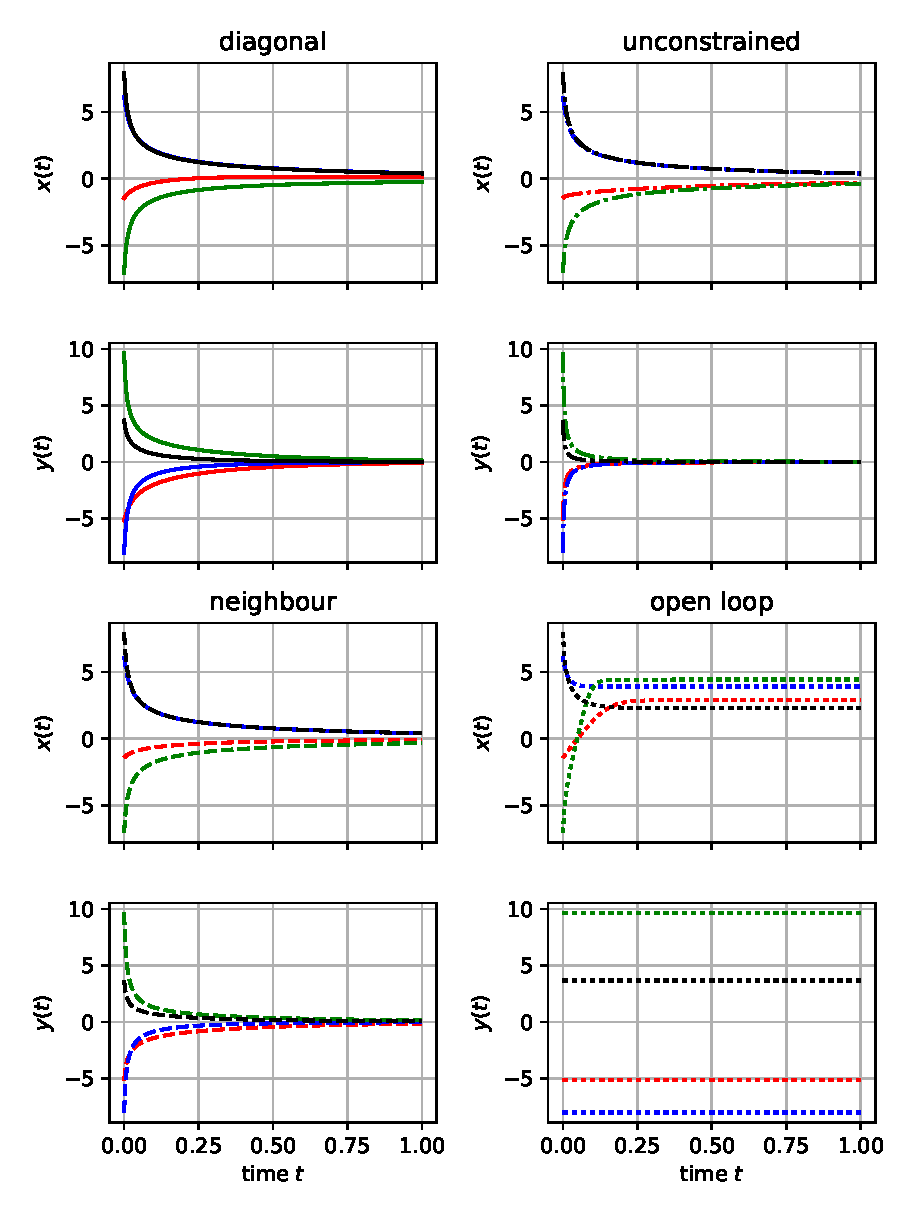
\includegraphics[width=\linewidth]{./imgs/simulation.eps}

	\caption{Simulation of network~\eqref{eq:example} with the target trajectory being the origin and under the controller obtained according to different constrains for the computation of $Y$: diagonal, neighbour and unconstrained. In contrast to these, the open loop simulation (performed with $u\equiv0$) does not converge to the origin.}
	\label{fig:3dsim}
\end{figure}

\begin{figure}[htbp!]
	\centering
%	\includegraphics[]{}
	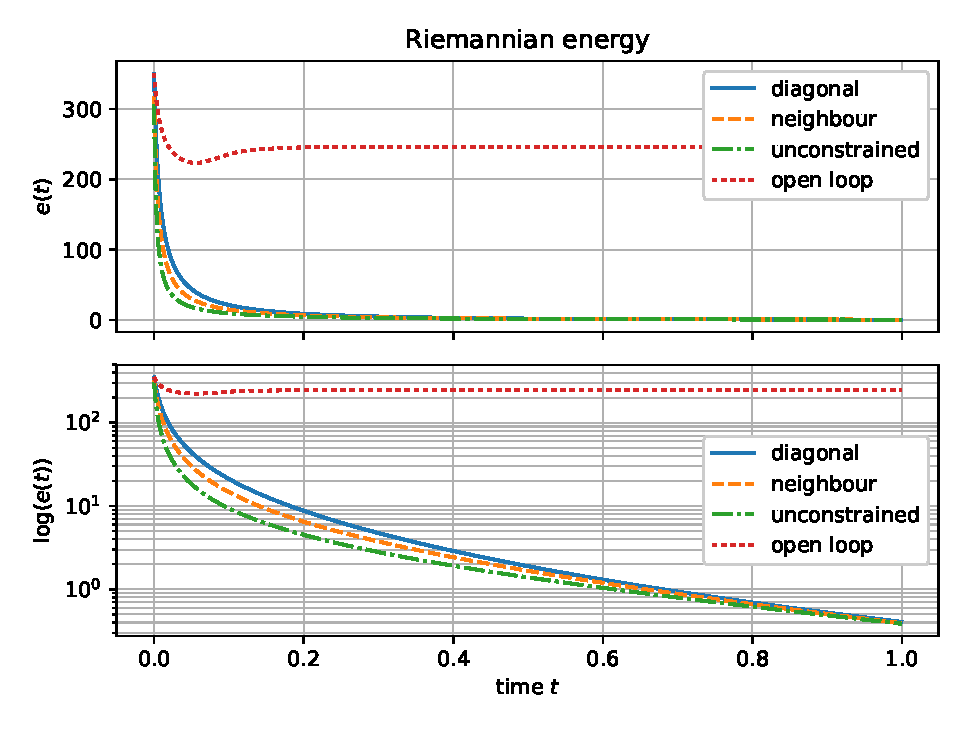
\includegraphics[width=\linewidth]{./imgs/Riemannian_energy.eps}
	\caption{Computation of the Riemannian energy along solutions to \eqref{eq:example}, according to each of each case. The bottom graph is the logarithm of the Riemannian energy.}
	\label{fig:Riemannian energy}
\end{figure}

\mypara When $N>8$ and $Y$ is a full-rank matrix with elements described by polynomials, the set of matrix inequalities~\eqref{eq:main result} could not be solved on a standard desktop computer. A reason for this issue is the dependence of each element of the matrix $Y$ on the variable $q$. Another reason is the need to verify if the matrix inequality~\eqref{eq:MI:SSCCM} is negative definite. For instance, when  polynomials with degree $d$ are employed, the number of monomials to be optimized in the $(i,j)$ position the matrix $T$ is
\begin{equation*}
		\begin{pmatrix}
n+d\\ d
\end{pmatrix}
\end{equation*}
\cite{Waki2006}. Consequently, when no structural constraints are imposed on $Y$, this verification can lead to
\begin{equation*}
n\dfrac{n+1}{2}\begin{pmatrix}
n+d\\ d
\end{pmatrix}
\end{equation*}
monomials to be computed. This motivates the approach proposed in this paper.

\mypara To show the advantages of the method proposed in this paper, a benchmark composed of  three scenarios, according to the constraints imposed on the matrix $Y$, has been created.  Namely, the unconstrained case, the ``neighbor'' case, and the fully decentralized case. For the two latter cases, it was possible to consider up to $N=256$ systems for the ``neighbor'' case and up to $N=512$ systems for the fully decentralized (diagonal) case. In these scenarios the techniques provided by chordal graphs have been employed.

\mypara In the first one, the graph $\mathscr{G}_c$ describing the communication network is fully connected, i.e., $\mathscr{E}_c=\mathbb{N}_{[1,4]}\times\mathbb{N}_{[1,4]}$ and no constraints were imposed on the matrix $Y$. Consequently, for each $i\in\mathbb{N}_{[1,4]}$, for every $j\in\mathbb{N}_{[1,4]}$, $Y_{ij}=Y_{ij}(q_1,\ldots,q_4)\in\mathbb{R}^{1\times 2}$.
	
The parser took 98  seconds to solve the set of matrix inequalities~\eqref{eq:main result}. The matrix $W$ is given by
\begin{equation*}
		W=\mathbin{\mathtt{diag}}(1,1,2,1,2,1,1,1)
\end{equation*}
and the matrix $Y$ has elements defined, for every $q\in\mathbb{R}^8$, by
\begin{align*}
	\overline{Y}_i(q)=&-2\begin{bmatrix}
	y_i&1+\sum_{k=1}^4 y_k^2+x_k^2
	\end{bmatrix},\\
	\hat{Y}_i(q)=&-\begin{bmatrix}y_i,&0\end{bmatrix},\\
	0_{1\times2}=&\begin{bmatrix}0,&0\end{bmatrix},
\end{align*}
where $i\in\mathbb{N}_{[1,4]}$, and structure given by the matrix
\begin{equation}\label{eq:example:Y:general}
		\resizebox*{0.85\columnwidth}{!}{$\begin{bmatrix}
			\overline{Y}_1(q),&0_{1\times 2},&-0.03\hat{Y}_1(q),&0_{1\times2}\\
			0_{1\times 2},&\overline{Y}_2(q),&0_{1\times 2},&-0.04\hat{Y}_2(q)\\
			-0.04\hat{Y}_3(q),&0_{1\times 2},&\overline{Y}_3(q),&0_{1\times 2}\\
			0_{1\times 2},&-0.03\hat{Y}_4(q),&0_{1\times 2},&\overline{Y}_4(q)
		\end{bmatrix}$}.
\end{equation}

\mypara For the remaining cases, the structure of the network composed of systems of the form \eqref{eq:example} has been exploited. More specifically, Proposition~\ref{prop:clique tree decomposition} can be employed, as the graph describing the interconnection of the network is a subclass of chordal graphs. Consequently, the MI~\eqref{eq:MI:SSCCM} can be decomposed into $N-1$ cliques  described by the matrix
\begin{equation*}
	F_k=\begin{bmatrix}
		F_{11}&F_{12}\\
		F_{12}^\top&F_{22}
	\end{bmatrix}\;.
\end{equation*}

\mypara In the ``neighbor'' case, the communication network topology $\mathscr{G}_c$ has the same structure as the network system. Consequently, the set of edges $\mathscr{E}_c$ is defined as $\mathscr{E}_c=\mathscr{E}_p$.

\mypara The time taken by the parser to solve the set of matrix inequalities~\eqref{eq:main result}, in this case, was 3.5 seconds. The matrix $W$ is given by
\begin{equation*}
		W=\mathbin{\mathtt{diag}}(2,1,1,1,1,1,2,1)
\end{equation*}
and the matrix $Y$ has the structure defined, over $q\in\mathbb{R}^8$ as
\begin{equation}\label{eq:example:Y:neighbor and decentralized}
	 Y(q)=\begin{bmatrix}
 	\overline{Y}_1(\cdot)&0_{1\times2}&0_{1\times2}&0_{1\times2}\\
 	0_{1\times2}&\overline{Y}_2(\cdot)&0_{1\times2}&0_{1\times2}\\
 	0_{1\times2}&0_{1\times2}&\overline{Y}_3(\cdot)&0_{1\times2}\\
 	0_{1\times2}&0_{1\times2}&0_{1\times2}&\overline{Y}_4(\cdot)
 \end{bmatrix}\;,
\end{equation}
with elements given, for every $(q_i,\breve{q}_i)\in\mathbb{R}^2\times\mathbb{R}^{\breve{n}_i}$, by 
\begin{equation*}
	\overline{Y}_i(q_i,\breve{q}_i)=-2\begin{bmatrix}
	y_i,&1+\sum_{j\in\mathscr{N}(i)}x_j^2+y_j^2)\end{bmatrix}, i\in\mathbb{N}_{[1,4]}\;.
\end{equation*}
 

\mypara In the fully decentralized case, the set of edges $\mathscr{E}_c$ is defined as $\mathscr{E}_c=\{(1,1),(2,2),(3,3),(4,4)\}$. The time taken by the parser to solve the set of matrix inequalities~\eqref{eq:main result} was 2.6 seconds, the matrix $W$ is given by
\begin{equation*}
 W=\mathbin{\mathtt{diag}}\left(2,1,1,1,1,1,1,1\right),\\
\end{equation*}
and the matrix $Y$ with structure given by \eqref{eq:example:Y:neighbor and decentralized} with elements defined, for every $q_i\in\mathbb{R}^2$, by 
\begin{align*}
 \overline{Y}_i(q_i)=-\begin{bmatrix}2y_i,3+2(x_i^2+y_i^2)\end{bmatrix},\quad i\in\mathbb{N}_{[1,4]}\;.
\end{align*}

\mypara Figure \ref{fig:time graph} shows a plot of the time taken by parser to the set of matrix inequalities~\eqref{eq:main result} for the three cases considered in this topology: unconstrained, ``neighbor'' and fully decentralized.  According to this graph, for $N=1,2$, the time taken by the parser to solve the set of matrix inequalities~\eqref{eq:main result} has the same order of magnitude for the three cases. However, as the number of systems increases, the unconstrained case takes more time to be solved than the ``neighbor'' case which, in turn, takes more time than the fully decentralized case. The time difference between the two latter cases can be explained by fact that, for the ``neighbor'' case, the matrix $Y$ contains more non-identically zero elements than the fully decentralized case. In addition to this, in the former case, each element is defined as a polynomial of second degree on the variables $q_i$ and $\breve{q}_i$, while for the latter, they are defined on the variable $q_i$ only.

\mypara Table~\ref{tab:chain case} shows a summary of the time taken by the solver to compute the matrices $W$ and $Y$ satisfying the set of matrix inequalities~\eqref{eq:main result}, according to the unrestricted, ``neighbor'' and fully decentralized cases.

\begin{figure}[htpb!]
	\centering
	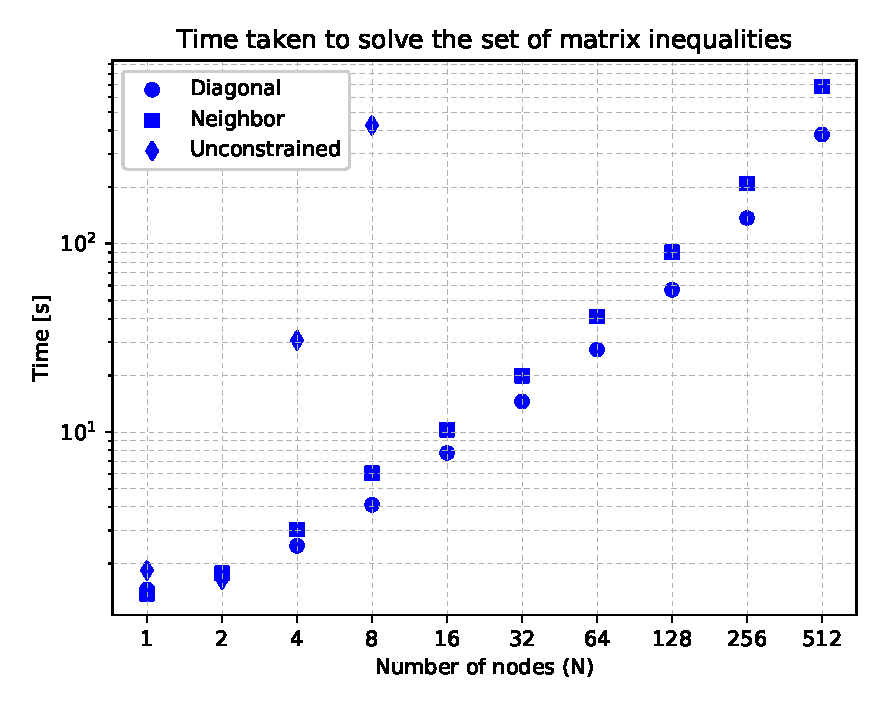
\includegraphics[width=\columnwidth]{./imgs/ParserTimes}\vspace{-2em}
	\caption{Time taken to solve the set of matrix inequalities~\eqref{eq:main result} for the three cases under consideration. The number of agents started with one system and doubled  until the maximum that the computer could process (8 for the unconstrained case, 256 for the ``neighbor'' case and 512 for the fully decentralized case). Axes are on log scale.}
	\label{fig:time graph}
\end{figure}

\begin{table}
	\begin{tabular}{r|c}
	Case&Time taken by the solver (4 agents)\\ \hline
	Unconstrained&98s\\
	Neighbor&3.5s\\
	Fully decentralized&2.6s\\\hline
	\end{tabular}\vspace{1em}
	\caption{A summary of the time taken to solve the set of matrix inequalities~\eqref{eq:main result} using chordal graph decomposition, in the topology illustrated by Fig.~\ref{fig:graph}.}
	\label{tab:chain case}
\end{table}

\mypara Regarding the on-line integration phase, since the matrices $W$ computed in each case are  constant, for each index $i\in\mathbb{N}_{[1,4]}$, the geodesic curve connecting the origin to a point $q_i\in\mathbb{R}^2$ is a straight line: $\gamma_i(s)=sq_i$, where $s\in[0,1]$. For each index $i\in\mathbb{N}_{[1,4]}$ and assuming that $u^\ast\equiv0$, the feedback law is  given by the formula
\begin{equation*}
	k= \int_0^1Y(sq)W^{-1}q\,ds.
\end{equation*}
Given the structure of the matrices $Y$ and $W$, each line $i\in\mathbb{N}_{[1,4]}$ is given by
\begin{equation*}
k_i=\begin{cases}
	\displaystyle\int_0^1Y_i(sq)W_i^{-1}q_i\,ds,&\text{if unconstrained}\\
	\displaystyle\int_0^1Y_i(sq_i,s\breve{q}_i)W_i^{-1}q_i\,ds,&\text{if ``neighbor''}\\
	\displaystyle\int_0^1Y_i(sq_i)W_i^{-1}q_i\,ds,&\text{if fully decentralized.}
\end{cases}
\end{equation*}
Moreover, from Theorem~\ref{thm:main result}, the feedback law $k$ solves Problem~\ref{problem formulation} for the network resulting from the interconnection of systems \eqref{eq:example}.

\subsection{A topology with a cycle}

\mypara The graph describing the network structure is provided in Figure~\ref{fig:cycle graph}. As in the Section~\ref{sec:chain topology}, here same three scenarios are considered. Namely, the unconstrained case, the ``neighbor'' case and the fully decentralized case.

\begin{figure}[htpb!]
	\centering
	\input{./imgs/NewExample.pdf_tex}
	\caption{Graph describing the network composed of systems of the form \eqref{eq:example}.}
	\label{fig:cycle graph}
\end{figure}

\mypara In the first scenario, the unconstrained case, the graph $\mathscr{G}_c$ describing the communication network is fully connected, i.e., $\mathscr{E}_c=\mathbb{N}_{[1,6]}\times\mathbb{N}_{[1,6]}$ and no constrained were imposed on the matrix $Y$. Consequently, the matrix $Y$ have elements given by $Y_{ij}=Y_{ij}(q_1,q_2,q_3,q_4)$, for each $i,j\in\mathbb{N}_{[1,4]}$, for each $(q_1,q_2,q_3,q_4)\in\mathbb{R}^8$.

\mypara The solver took 48s to solve the set of matrix inequalities~\eqref{eq:main result}. The matrix $W$ obtained is given by
\begin{equation*}
	W=\mathbin{\mathtt{diag}}(0.1,1,0.1,1,0.1,1,0.1,1,0.1,1,0.3,1).
\end{equation*}
The matrix $Y$ is given by
\begin{equation*}
	\begin{bmatrix}
		\overline{Y}_{11}(q)&0_{1\times2}&0_{1\times2}&0_{1\times2}&0_{1\times2}&0_{1\times2}\\
		0_{1\times2}&\underline{Y}_{22}(q)&0_{1\times2}&0_{1\times2}&0_{1\times2}&0_{1\times2}\\
		0_{1\times2}&0_{1\times2}&\overline{Y}_{33}(q)&0_{1\times2}&0_{1\times2}&0_{1\times2}\\
		0_{1\times2}&0_{1\times2}&0_{1\times2}&\overline{Y}_{44}(q)&0_{1\times2}&0_{1\times2}\\
		0_{1\times2}&0_{1\times2}&0_{1\times2}&0_{1\times2}&\overline{Y}_{55}(q)&0_{1\times2}\\
		0_{1\times2}&0_{1\times2}&0_{1\times2}&0_{1\times2}&0_{1\times2}&\underline{Y}_{66}(q)
	\end{bmatrix},
\end{equation*}
for every $q\in\mathbb{R}^{12}$, where 
\begin{align*}
 \overline{Y}_{ij}(q)=&\ -\begin{bmatrix}3y_i,&4+4\sum_{i=1}^6(x_i^2+y_i^2)\end{bmatrix},\\
 \underline{Y}_{ij}(q)=&\ -\begin{bmatrix}3y_i,&2+2\sum_{i=1}^6(x_i^2+y_i^2)\end{bmatrix},
\end{align*}
for each index $i,j\in\mathbb{N}_{[1,6]}$.

\mypara In the ``neighbor'' case, the topology of the controller is the same as of the network. More precisely, $\mathscr{G}_c=\mathscr{G}_p$. The solver took 57s to solve the set of matrix inequalities~\eqref{eq:main result}.

\mypara The matrix $W$ obtained is given by
\begin{equation*}
	W=\mathbin{\mathtt{diag}}(1,1,1,1,1,1,1,1,1,1,2,1).
\end{equation*} 
The matrix $Y$ is given by Equation~\eqref{eq:Y mixed case:neighbor}.

\setcounter{MaxMatrixCols}{20}
\begin{figure*}
\begin{equation}\label{eq:Y mixed case:neighbor}
	\resizebox{.9\textwidth}{!}{
$-\begin{bmatrix}
		2y_1&4+3(|q_1|^2+|\breve{q}_1|^2)&0&0&0&0&0&0&0&0&0&0\\
		0&0&2y_2&2+2(|q_2|^2+|\breve{q}_2|^2)&0&0&0&0&0&0&0&0\\
		0&0&0&0&2y_3&4+3(|q_3|^2+|\breve{q}_3|^2)&0&0&0&0&0&0\\
		0&0&0&0&0&0&2y_4&3+3(|q_4|^2+|\breve{q}_4|^2)&0&0&0&0\\
		0&0&0&0&0&0&0&0&2y_5&4+3(|q_5|^2+|\breve{q}_5|^2)&0&0\\
		0&0&0&0&0&0&0&0&0&0&2y_6&4+3(|q_6|^2+|\breve{q}_6|^2)
	\end{bmatrix}$}
\end{equation}
\end{figure*}

\mypara In the last scenario, the fully decentralized case, the set of edges $\mathscr{E}_c$ of the graph $\mathscr{G}_c$ is specified as $\mathscr{E}_c=\{(1,1),(2,2),(3,3),(4,4)\}$ and no constrained were imposed on the matrix $Y$. The solver took 43s to solve the set of matrix inequalities~\eqref{eq:main result}.

\mypara The matrix $W$ obtained is given by
\begin{equation*}
	W=\mathbin{\mathtt{diag}}(0.6,1,0.8,1,0.6,1,0.4,1,0.7,1,1,1)
\end{equation*}

\mypara The matrix $Y$ have elements given by $Y_{ij}=Y_{ij}(q_i)\delta_{ij}\in\mathbb{R}^{2\times 1}$, for each $i,j\in\mathbb{N}_{[1,6]}$, and for each $q_i\in\mathbb{R}^{2}$, where $\delta_{ij}$ is the Kronecker's delta. More specifically, the matrix $Y$ is presented in Equation~\eqref{Y for mixed case}.

\begin{figure*}
\begin{equation}\label{Y for mixed case}
	Y=-\begin{bmatrix}
	2y_1&5+3|q_1|^2&0&0&0&0&0&0\\
 	0&0&2y_2&3+2|q_2|^2&0&0&0&0\\
 	0&0&0&0&2y_3&5+3|q_3|^2&0&0\\
 	0&0&0&0&0&0&2y_4&4+2|q_4|^2
	\end{bmatrix}
\end{equation}
\end{figure*}

\begin{table}
	\begin{tabular}{r|c}
	Case&Time taken by the solver (4 agents)\\ \hline
	Unconstrained&48s\\
	Neighbor&57s\\
	Fully decentralized&43s\\\hline
	\end{tabular}\vspace{1em}
	\caption{A summary of the time taken to solve the set of matrix inequalities~\eqref{eq:main result} using chordal graph decomposition, in the topology illustrated by Fig.~\ref{fig:cycle graph}.}
	\label{tab:mixed example}
\end{table}

\section{Conclusion}\label{sec:Conclusion}

\mypara In terms of semidefinite programming, employing control contraction metrics allows one to formulate the search for the controller as a convex optimization problem. Although this is one of its main advantages over the search of control-Lyapunov functions, it cannot handle systems with a large number of states, in general.

\mypara For large-scale systems, the approach presented in this paper exploits sparsity to design feedback laws with a prescribed structure. More precisely, during the off-line phase, by imposing a block-diagonal structure on the matrix describing the metric, a controller with a prescribed structure can be synthesized. Moreover, the on-line integration phase computation can be in parallel, because each block defines a metric to the corresponding component of the state space.

\appendices


% Can use something like this to put references on a page
% by themselves when using endfloat and the captionsoff option.
\ifCLASSOPTIONcaptionsoff
  \newpage
\fi



% trigger a \newpage just before the given reference
% number - used to balance the columns on the last page
% adjust value as needed - may need to be readjusted if
% the document is modified later
%\IEEEtriggeratref{8}
% The "triggered" command can be changed if desired:
%\IEEEtriggercmd{\enlargethispage{-5in}}

% references section

% can use a bibliography generated by BibTeX as a .bbl file
% BibTeX documentation can be easily obtained at:
% http://mirror.ctan.org/biblio/bibtex/contrib/doc/
% The IEEEtran BibTeX style support page is at:
% http://www.michaelshell.org/tex/ieeetran/bibtex/
%\bibliographystyle{IEEEtran}
% argument is your BibTeX string definitions and bibliography database(s)
%\bibliography{IEEEabrv,../bib/paper}
%
% <OR> manually copy in the resultant .bbl file
% set second argument of \begin to the number of references
% (used to reserve space for the reference number labels box)
%\printbibliography

\bibliographystyle{ieeetr}
\bibliography{Library,Distributed}

\end{document}


